%%=============================================================================
%% Methodologie
%%=============================================================================

\chapter{\IfLanguageName{dutch}{Proof of concept}{Proefafdruk}}
\label{ch:Proof of concept}

Het doel van dit hoofdstuk is om een idee te creëren van de omgeving waarin Cisco Identity Services Engine is geïmplementeerd. Hierbij is een uitgebreide uitleg over de elementen die aanwezig zijn binnen de omgeving van Cisco terug te vinden in dit hoofdstuk. Ieder hardware apparaat is zorgvuldig beschreven, onder andere is er informatie te vinden over de specificatie, de configuraties en de instellingen van de hardware componenten. Daarnaast zijn ook de implementaties van de virtuele machines verder toegelicht.
\newline
\newline
Samen met deze informatie zijn belangrijke schema’s weer verwerkt in dit hoofdstuk, die een visueel beeld geven over dit afgezonderd netwerk. 
Vervolgens is er de sectie die de enquête bespreekt. De enquête bespreking bevat voornamelijk informatie die terug te vinden in de sectie \ref{sec:enquête}. 

\section{Cisco Identity Services Engine omgeving}

Voor de implementaties en testen van Cisco Identity Services Engine en zijn benodigde use cases is er een omgeving vereist. Deze omgeving is voorzien door een Belgische aanbieder van digitale televisie, breedband-internet, mobiele telefonie, enz. Deze Belgische aanbieder staat gekend als Telenet Group N.V. Implementaties en de testen van Cisco Identity Services Engine en met zijn benodigde use cases is uitgewerkt in een Telenet thuisnetwerk.
\newline
Zoals elk thuisnetwerk dat voorzien is door een Belgische internet aanbieder bevat het thuisnetwerk een aantal Telenet Access Points en een Telenet modem. De kabelverbinding die data verzend vanuit de Telenet centrale naar de Telenet modem is een coaxkabel. Het is dankzij de coaxkabel dat het thuisnetwerk verbonden is met het Wide Area Network (ook gekend als WAN).
\newline
\newline
Om de essentiële componenten van dit thuisnetwerk te beschermen tegen breuk, is de implementatie verder uitgewerkt in een afgezonderd netwerk. Dit wordt mogelijk gemaakt met behulp van een virtuele opensource router/firewall zoals Pfsense. Dit virtuele routerje dient als gateway voor de verschillende vlan’s waarbij het thuisnetwerk gebruikt zal worden als ‘uplink’ naar het internet. 

\subsection{Server VMware ESXi}
Het afgezonderd netwerkje bestaat uit een rack server waarop een viertal virtuele machines draaien. Deze virtuele machine zijn: Cisco Identity Service Engine, het virtuele routerje, genaamd Pfsense en twee  Windows Server 2019 datacenters machines. Dit wordt eenvoudig weergegeven in figuur \ref{fig:vms} die de virutele machines weergeeft. De creatie van deze virtuele machines is mogelijk gemaakt door VMware ESXi. VWware ESXi is een type-1 hypervisor van enterprise-klasse, ontwikkeld door VMware voor het inzetten en bedienen van virtuele machines. 
\newline
\newline
De ESXi server is geconfigureerd door het gebruik van een ‘bootable usb’. Deze bootable usb bevatte al nodige software om de server te voorzien met VMware ESXi. Vervolgens werd de server geconfigureerd met een aantal belangrijke settings, zoals het instellen van een IP adres, subnet mask, raid controller, enz. Waarbij zijn volgende settings voorzien op deze ESXi server: 

\begin{itemize}
	\item IP adres: 192.168.0.183
	\item Subnet: 255.255.255.0
	\item Default gateway: 192.168.0.1
	\item raid controller: RAID 10
\end{itemize}

\begin{figure}[H]
	\centering
	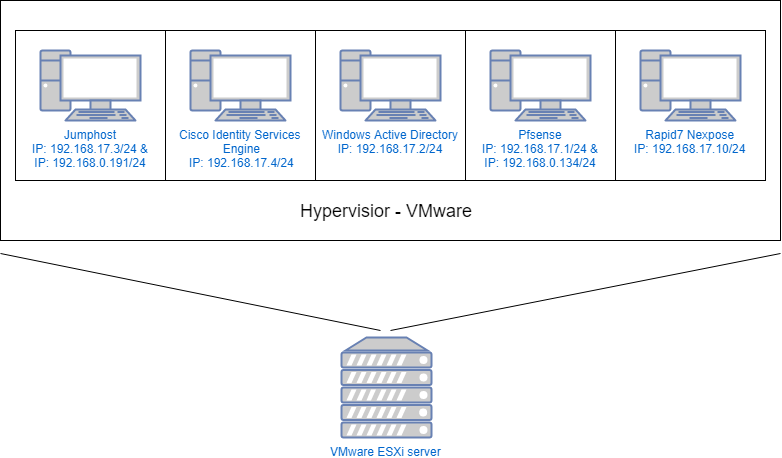
\includegraphics[height=0.3\textheight]{servervm.png}
	\caption{Virtuele machines in VMware ESXi server}
	\label{fig:vms}
\end{figure}

\newpage
Door de configuratie van deze IP instellingen, is de VMware ESXi server toeganglijk via de webbrowser. Virtuele machines kunnen via de webbrowser beheerd, verwijderd en gecreëerd worden. Daarnaast werd de hard disk drive ingesteld met een RAID controller. RAID, een afkoring voor Redundant array of independent disks is een dataopslagtechnologie waarbij meerdere harde schijven gecombineerd worden tot één of meer logische virtuele opslageenheden. Dit heeft als doel om de veiligheid, snelheid en de capaciteit te kunnen vergroten. Hierbij is op de VMware ESXi RAID 10 geconfigueerd. RAID 10 is een hybride combinatie tussen RAID 1 en RAID 0. Waarbij men de snelheid van striping met de veiligheid van mirroring combineert. 
\newline
\newline
Dit is de veiligste en snelste methode maar ook de duurste. Het is een dure methode omdat er gebruik wordt gemaakt van RAID 1, dus voor iedere 1TB aan opslagruimte is er ook 1TB aan mirror ruimte nodig, in combinatie met RAID 0 waardoor er veel fysieke harde schijven nodig zijn. In figuur \ref{fig:Raid10} wordt een voorbeeld van een RAID 10 schema weergegeven.

\begin{figure}[H]
	\centering
	\includegraphics[height=0.25\textheight]{Raid10.png}
	\caption{Voorbeeld configuratieschema RAID 10 (\cite{Raid10}).}
	\label{fig:Raid10}
\end{figure}

Vervolgens zijn er in de VMware ESXi server opstelling drie van de vier fysieke ethernet adapters gebruikt. Deze adapters zijn op hun beurt verbonden met een virtuele switch. Elk van de fysieke adapters heeft een andere functie die weergegeven zijn in de onderstaande lijst. 

\begin{itemize}
	\item vmnic0,is de fysieke adapter die verbonden is met de virtuele switch, genaamd 'VSwitch0'.
	\item vmnic2,is de fysieke adapter die verbonden is met de virtuele switch, genaamd 'Sub\textunderscore switch'.
	\item vmnic3,is de fysieke adapter die verbonden is met de virtuele switch, genaamd 'Cisco \textunderscore switch'.
\end{itemize}

\newpage
\subsubsection{Virtuele switches}
\subsubitem{\bf VSwitch0}
\newline
De 'VSwitch0' is een virtuele switch die voorzien is om de VMware ESXi server te contacteren via de webbrowser. Op figuur \ref{fig:Vswitch0} ziet men dat de 'VSwitch0' is ingesteld met vlan id 0, dat geen vlan identificatie voorziet. 
\newline
\newline
Data passeert deze interface wanneer gebruikers surfen naar "https://192.168.0.183". Vervolgens passeert de data langs de fysieke poort vmnic0 die data doorgeeft aan de VSwitch0. Wanneer data terecht komt op de VSwitch0, stuurt hij op zijn beurt de data door naar de VMKernel poort.

\begin{figure}[H]
	\centering
	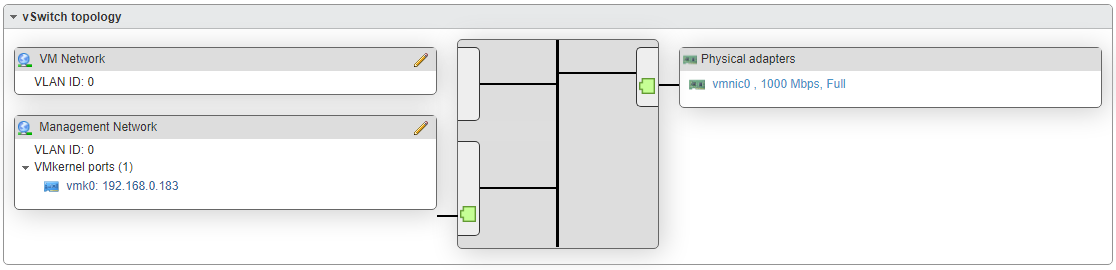
\includegraphics[width=0.7\textwidth]{VSwitch0.png}
	\caption{Topologie van de 'VSwitch0'}
	\label{fig:Vswitch0}
\end{figure}

\subsubitem{\bf Sub\textunderscore switch}
\newline
Op figuur \ref{fig:subswitch} ziet men dat de 'Sub\textunderscore switch' een virtuele switch is die gebruikt wordt voor WAN interface van de Pfsense. De Wide Area Network interface voorziet data overdracht van het thuisnetwerk naar het afgezonderd LAN netwerk. Hierdoor is connectie met het afgezonderd netwerk mogelijk via deze interface. Bovendien wordt deze virtuele switch ook gebruikt door de jumphost om remote desktop protocol connecties te maken met de virtuele machines binnen het afgezonderd LAN netwerk. 

\begin{figure}[H]
	\centering
	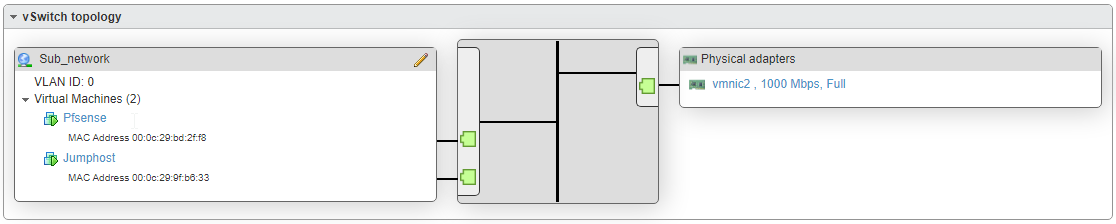
\includegraphics[width=0.7\textwidth]{Subswitch.png}
	\caption{Topologie van de 'Sub\textunderscore switch'}
	\label{fig:subswitch}
\end{figure}
\newpage
\subsubitem{\bf Cisco\textunderscore switch}
\newline
Ten slot is er de 'Cisco\textunderscore switch' die gebruikt wordt om connectie te maken met alle apparaten achterliggend de fysieke Cisco switch. Wanneer eind apparaten met de Cisco switch verbinden, dan zal de data passeren via de 'Cisco\textunderscore switch'. Bovendien is op figuur \ref{fig:Ciscoswitch} te zien dat alle virtuele machines zich in deze omgeving bevinden. Dit zorgt er voor dat de Cisco\textunderscore switch ingesteld is met vlan id 10, waarbij enkel data vanuit vlan 10 wordt doorgestuurd naar de voorziene eind apparaten.

\begin{figure}[H]
	\centering
	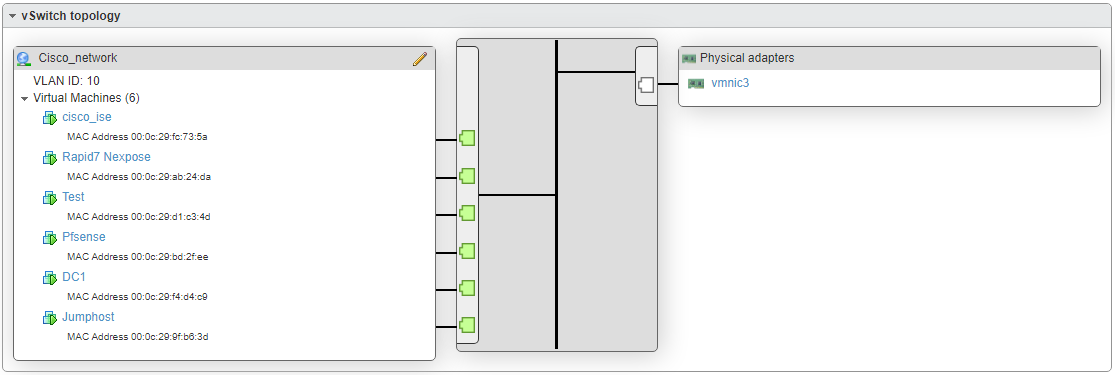
\includegraphics[width=0.7\textwidth]{CiscoSwitch_vmware.png}
	\caption{Topologie van de 'Cisco\textunderscore switch'}
	\label{fig:Ciscoswitch}
\end{figure}

\subsubsection{Server ESXi specificaties}
De VMware ESXi server is van het merk International Business Machines Corporation, gekend als IBM. Deze server werd oorsprongelijk gebruikt in de productie omgeving van Axians, maar wordt sinds kort als test server gebruikt. In figuur \ref{fig:VmwareSer} ziet men een afbeelding van de IBM ESXi server.
\newline
\newline
Het model van de VMware ESXi server is ‘System x3350 M3’ dat gekend staat binnen Axians als ‘de oude shr-esx-04 server’. De IBM ‘System x3350 M3’ bevat volgende specificaties:

\begin{itemize}
	\item Vormfactor: 1U Rack
	\item Processor:
	\begin{itemize}
		\item Proccessorsnelheid: 2.53GHz
		\item Processor: 6-core processor
	\end{itemize}
	\item Geheugen:
	\begin{itemize}
		\item Intern geheugen: 240 GB Random Access Memory
		\item Intern geheugentype: Double Data Rate 3 Synchronous Dynamic Random-Access Memory, gekend als DDR3 SDRAM
	\end{itemize}
	\item Opslag:
	\begin{itemize}
		\item Maximum aantal schrijven: 8 Slots
		\item Opslag: 4 Terabyte HHD 7500 RPM
	\end{itemize}
	\item Netwerk
	\begin{itemize}
		\item Ethernet interface type: Gigabit Ethernet
		\item Aantal ethernet poorten: 4 
	\end{itemize}
\end{itemize}

\begin{figure}[H]
	\centering
	\includegraphics[width=0.5\textwidth]{serveresxi.png}
	\caption{Foto van de ESXi VMware server}
	\label{fig:VmwareSer}
\end{figure}

\subsection{Cisco switch}
Naast de VMware ESXi server, bestaat de Cisco Identity Services Engine omgeving ook uit een Cisco switch. Dankzij een aantal configuraties op de Cisco switch kan de Cisco Identity Services Engine virtuele machine communiceren met de fysieke switch. Deze noodzakelijke configuraties speelden een belangrijke rol in de configuratie van de 'Port-based network access control' use case. 
\newline
\newline
Door een aantal basis configuraties op deze switch uit te voeren wordt communicatie tussen het afgezonderd netwerk en de eind apparaten die zich achter de Cisco switch bevinden ook mogelijk. Deze informatie is terug te vinden in de sectie \ref{sec:config}.

\subsubsection{Configuratie}
\label{sec:config}
Als eerst zijn een aantal commando's uitgevoerd die het netwerk apparaat beveiligen met een secret, line passwords en password encryption om inbreuk tegen te gaan. Vervolgens werd Gigabit Ethernet 0/1 geconfigureerd met de gepaste trunk settings om de gobale communicatie mogelijk te maken. Een trunk configuratie maakt data overdracht van de verschillende vlan's mogelijk. Volgende twee trunk commando's zijn hiervoor uitvoerd: 

\begin{itemize}
	\item switchport mode trunk
	\item switchport trunk allow vlan 10 
\end{itemize}

Gigabit Ethernet 0/1 werd rechtsverbonden met één van de interfaces op de VMware ESXi server, waarbij de virtuele switch ingesteld werd met vlan id 0 dat gelijk staan aan geen vlan identificatie. Vervolgens werd
op de Cisco switch vlan 10 gecreeërd met ip adres '192.168.17.5' en met subnet mask '255.255.255.0'. Vermits de interface Gigabit Ethernet 0/1 geconfigureerd is om verbinding te maken met de VMware ESXi server, zijn de overige interfaces bedoeld voor de communicatie met de eind apparaten. 
\newline
\newline
Om de 'Port-based network access control' use case te implementeren, werd een nieuw AAA model ingesteld. Dit AAA model werd vervolgens geïnitialiseerd met een radius server die gelijk staat aan het Internet Protocol adres van Cisco Identity Services Engine. Ten slotte werd de dot1x aaa authentication methode met zijn standaard netwerk groep mee configureerd. 
\newline
\newline
Om de configuraties van de Cisco switch te beëindeigen, werd dot1x system-auth-control vastgelegd en werden alle poorten voorzien van de nodige 'Port-based access control' configuraties. Figuur \ref{fig:RunningConfig} toont de running config van de Switch Cisco, daarnaast zijn alle nodige commando's in onderstaande lijst ook weergegeven.
\begin{itemize}
	\item \#enable
	\item \#config t
	\item (config)\#aaa new-model
	\item (config)\#aaa group server radius ISE
	\item (config-sg-radius)\#server-private 192.168.17.4 key Admin2020
	\item (config-sg-radius)\#exit
	\item (config)\#aaa authentication dot1x
	\item (config)\#aaa authorization network default group ISE
	\item (config)\#dot1x system-auth-control
	\item (config)\#interface range gig0/2-12
	\item (config-if-range)\#switchport mode access
	\item (config-if-range)\#switchmode access vlan 10
	\item (config-if-range)\#authentication host-mode multi-host
	\item (config-if-range)\#authentication port-control auto
	\item (config-if-range)\#dot1x pae auth
	\item (config-if-range)\#end
\end{itemize}

\begin{figure}[H]
	\centering
	\subfloat{{\includegraphics[width=3cm]{Switch_config1.png} }}%
	\qquad
	\subfloat{{\includegraphics[width=3cm]{Switch_config2.png} }}%
	\qquad
	\subfloat{{\includegraphics[width=3cm]{Switch_config3.png} }}%
	\caption{Running config van de Cisco switch}%
	\label{fig:RunningConfig}%
\end{figure}
Verder zijn 1G cat5e ethernet kabels gebruikt om de hardware componenten met elkaar te laten communiceren. De Unshielded Twisted Pair Ethernet kabels halen snelheden tot 1000 Mbit/s met een doorvoersnelheid van 100mhz. Wat geschikt is voor dit afgezonderd netwerk.

\subsubsection{Cisco switch specificaties}
De Cisco switch behoord tot de ‘Catalyst 2960-CX’ series die nu gekend staat binnen Axians als de ‘Demo switch’. Hierbij vindt men in onderstaande lijst de specificaties van de Cisco Catalyst 2960-CX serie switch:

\begin{itemize}
	\item Power over Ethernet:
	\begin{itemize}
		\item Ondersteunend: Ja
		\item Standaard: 802.3at (PoE+)
	\end{itemize}
	\item Netwerk:
	\begin{itemize}
		\item 8 Gigabit Ethernet aansluitingen
		\item 2 Gigabit Ethernet Copper uplinks
		\item 2 Gigabit Ethernet Small form-factor pluggable uplinks, gekend als SFP
	\end{itemize}
	\item Besturingsysteem/software:
	\begin{itemize}
		\item OS: Cisco IOS
    \end{itemize}
\end{itemize}


\subsection{Virtuele machines}
\subsubsection{Cisco Identity Services Engine}
De eerste virtuele machine waarop dieper wordt op ingegaan is Cisco Identity Services Engine. Deze virtuele machine zal zich verdiepen in de use cases: 'Port-based network access control', 'Policy-based network access control' en 'Thread-centric network access control'. Daarvoor zijn een aantal configuraties uitgevoerd op de virtuele machine van Cisco Identity Services Engine om een antwoord te geven het onderzoek. Hieronder worden de configuraties opgesplitst per use cases, waarbij de use cases vaak in de praktijk worden gecombineerd. De resultaten van de Cisco Identity Services Engine configuraties vindt men terug in Hoofdstuk \ref{ch:Resultaten}.
\newline
\newline
Alvorens men dieper ingaat op de use cases werd Cisco Identity Services Engine toegevoegd aan het Active Directory Domein. Figuren \ref{fig:AD_Cisco1} en \ref{fig:AD_Cisco2} tonen aan dat de virtuele machine van Cisco Identity Services Engine probleemloos toegevoegd is aan het domein 'Bachelorproef.com'. Dit toont aan dat Cisco Identity Services Engine eenvoudig geïntegreerd kan worden met een domein, waarbij in de toekomst extra policy rules kunnen ingevoerd worden. Dit onderzoek focust zich op de bescherming van de vrije interfaces op de Cisco switch door een extra authenticatie methode te voorzien en dus niet op integratie van 'Port-based network access control' het gebruik Active Directory Domein users.

De installatie van Cisco Identity Services Engine werd mogelijk gemaakt door \cite{CiscoISE_InstallationGuide}.

\begin{figure}[H]
	\centering
	\includegraphics[width=0.9\textwidth]{AD_ise.png}
	\caption{Cisco ISE gelinkt met het AD domein}%
	\label{fig:AD_Cisco1}%
\end{figure}

\begin{figure}[H]
	\centering
	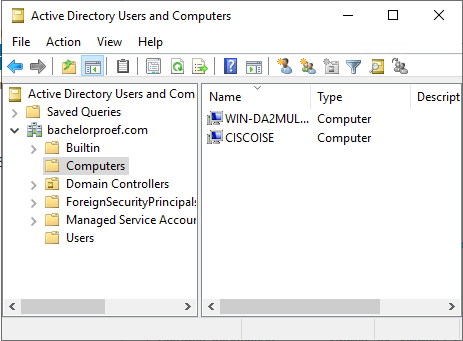
\includegraphics[width=0.7\textwidth]{ADComputers.png}
	\caption{Active Directory Users en Computers}
	\label{fig:AD_Cisco2}
\end{figure}
 \subsubitem{\textbf{Port- en Policy-based network access control }}
 \newline
 	Eerder werd vernoemd in sectie \ref{sec:config} dat voor implementatie van 'Port-based network access control' configuraties op de Cisco switch verplicht zijn. Op dit onderdeel van de sectie ligt de focus op de configuratie van de 'Port-based network access control' use case in de Cisco Identity Services Engine webbrowser. 
 	\newline
 	\newline
 	De Configuratie wordt gestart met de creatie van een aantal Cisco Identity Services Engine users in het 'Identity Management' tablad. In figuur \ref{fig:users} ziet men twee aangemaakte users waarbij user 'TestV2' zich in de groep 'Employees' bevindt en user 'Test' niet. Dit zal zich uiten wanneer een gebruiker zich aanmeldt met user 'Test' dan zal hij geen toegang krijgen tot het netwerk aan de hand van een policy rule.
 	
 	\begin{figure}[H]
 		\centering
 		\includegraphics[width=0.9\textwidth]{Port_users.png}
 		\caption{Cisco Identity Services Engine users}%
 		\label{fig:users}%
 	\end{figure}
 	
 	Vervolgens werd in het tablad 'Network Resources' de Cisco switch vastgelegd waardoor Cisco Identity Services Engine communicatie met het netwerk apparaat kan vaststellen. Figuur \ref{fig:ISESwitch} toont de configuratie voor deze communicatie. 
 	
 	 	\begin{figure}[H]
 		\centering
 		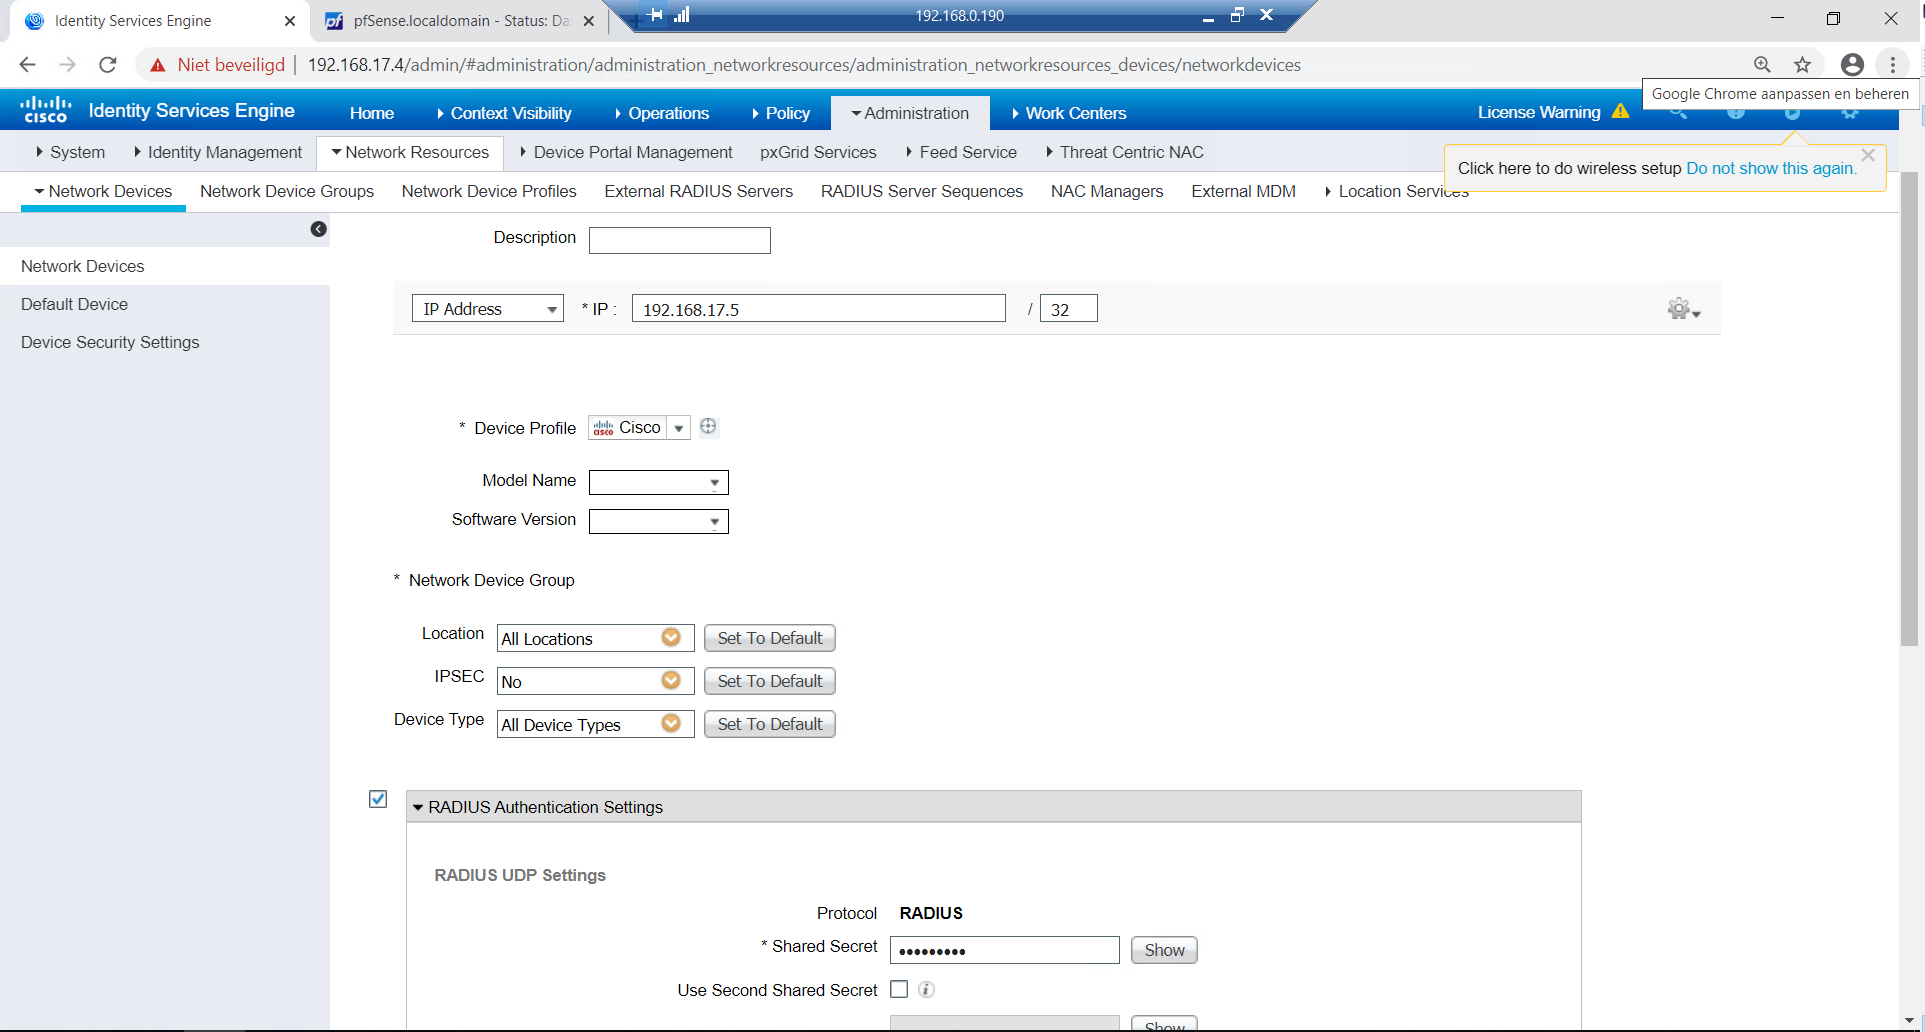
\includegraphics[width=0.7\textwidth]{ISESwitch.png}
 		\caption{Configuratie van de Cisco switch in ISE}%
 		\label{fig:ISESwitch}%
 		\end{figure}
 	
 	Ten slotte is een policy rule ingesteld waarbij gecontroleerd wordt of de gegevens overeenkomen met de instellingen van de policy rule. In dit geval laat de policy rule netwerk trafiek tot als de gebruiker de juiste identificatie gegevens ingeeft maar anderzijds ook wanneer de gebruiker zich in de groep 'Employees' bevindt. Op figuur \ref{label} is policy role weergegeven.
 	
	 	 \begin{figure}[H]
		\centering
		\includegraphics[width=0.7\textwidth]{PolicySet_Port.png}
		\caption{Configuratie van de 802.1x policy rule in ISE}%
		\label{fig:ISESwitch}%
		\end{figure}

 \subsubitem{\textbf{Thread-centri- en Policy-based network access control }}
  \newline
	!!!TO DO!!! Lorem ipsum dolor sit amet, consectetur adipiscing elit. Sed sed euismod velit, sed hendrerit justo. Praesent a hendrerit diam, ut imperdiet enim. In placerat nisl et commodo laoreet. Nullam convallis semper nibh nec cursus. Pellentesque a urna iaculis, eleifend turpis sit amet, varius velit. Nulla vitae est euismod, feugiat sem quis, fringilla nibh. Quisque ornare orci nisl, non pretium felis tempor id. Proin varius fermentum velit eu imperdiet. Praesent quis dolor at metus ornare dignissim sed finibus mauris. Maecenas pellentesque, ante ac vulputate dapibus, nisl nisi tristique libero, eu sollicitudin dolor est nec quam. Sed in lobortis sem. Phasellus nec diam eu magna lacinia tincidunt vitae in elit.
 
Verder werd systeem geïnstalleerd op een Red Hat Enterprise 7 distributie, waar vogende specificaties voor werd vrijgemaakt: 

\begin{itemize}
	\item Geheugen: 128 GB Random Access Memory
	\item Opslag: 512 GB
	\item CPU: 24 cores
	\item Netwerk adapter: Cisco\textunderscore netwerk
\end{itemize}

\subsubsection{Windows server 2019 datacenter}
Het gebruik van een Windows Server 2019 maakt de creatie van een Active Directory domein mogelijk. Een nieuwe forest werd hiervoor aangemaakt en de Windows Server 2019 werd meteeon ook gepromoveerd naar de domeincontroller binnen het 'bachelrorproef.com' netwerk.
\newline
\newline
Via Cisco Identity Service Engine kan men subset van domeinen selecteren vanuit de vertrouwde domeinen voor authenticatie en autorisatie. Deze subset van domeinen worden authenticatiedomeinen genoemd. Het definiëren van deze authenticatiedomeinen verbetert de beveiliging door bepaalde domeinen te blokkeren, waardoor de authenticatie van de gebruikers op deze domeinen wordt beperkt.
\newline
\newline
Zoals voorheen vermeld is integratie met Windows Server Active Directory en Cisco Identity Services Engine reeds mogelijk. Hierdoor kunnen bedrijven met Cisco Identity Services opteren om werknemers te laten inloggen op het netwerk met de 'Domain Users. Vaak wordt deze methode geïntegreerd met het 'wireless' aanmelden op netwerk door gebruik van de Active Domain Directory gegevens. Helaas beschikte dit afgezonderde netwerk niet over een wireless controller die dit mogelijk maakt. Cisco Identity Services voorziet hiervoor vooraf gedefinieerde regels.

Verder wordt het ‘Remote Desktop Protocol (RDP)’ in combinatie met het Internet Protocol (IP) adres gebruikt om de Windows machines te bereiken.
\newline
\newline
Om de Windows server 2019 datacenter te gebruiken werden volgende specificaties vrijgemaakt:

\begin{itemize}
	\item Geheugen: 16 GB Random Access Memory
	\item Opslag: 126 GB
	\item CPU: 20 cores
	\item Netwerk adapter: Cisco\textunderscore netwerk
\end{itemize}

Als laatstse werd de installatie van Windows Server 2019 datacenter mogelijk gemaakt door \cite{Win19_InstallationGuide}. 

\subsubsection{Pfsense}
De Pfsense virtuele machine verwijst naar de virtuele router waarbij één interface van de Pfsense gebruikt wordt als gateway voor alle vlan’s en van alle componenten die zich achter de Cisco switch bevinden. Vervolgens wordt de WAN interface van de Pfsense gebruikt om de data van en naar de Local Area Network interface te sturen. Hierdoor is communicatie vanuit het thuisnetwerk met het afgezonderd netwerk mogelijk.
\newline
\newline
De pfsense is enkel te contacteren binnen het afgezonderd netwerk door het ‘Hypertext Transfer Protocol (HTTP)’ te gebruiken. Met andere woorden kunnen enkel machines in het netwerk '192.168.17.0/24' de Pfsense interface bereiken door te surfen naar het ip adres: '192.168.17.1'. Op figuur \ref{fig:Pfsense} is te zien dat de home interface van de Pfsense te bereiken is via 'http://192.168.17.1/'.
\newline
\newline
Ten slotte werd dit systeem geïnstalleerd op een Free Berkeley Software Distribution, waar volgende specificaties zijn voor vrijgemaakt: 

\begin{itemize}
	\item Geheugen: 4 GB Random Access Memory
	\item Opslag: 25 GB
	\item CPU: 4 cores
	\item Netwerk adapter: Cisco\textunderscore netwerk
\end{itemize}
De installatie van Pfsense werd mogelijk gemaakt door \cite{Pfsense_InstallationGuide}.

\begin{figure}[H]
	\centering
	\includegraphics[width=0.7\textwidth]{PfsenseHome.png}
	\caption{Home interface Pfsense}
	\label{fig:Pfsense}
\end{figure}

\subsubsection{Jumphost}
Een jumphost is een tussenliggende host machine waarbij connectie naar een extern netwerk mogelijk is. Vervolgens kan een verbinding worden gemaakt met een andere host in het extern netwerk. Met andere woorden 'jumpt' men dus van het ene apparaat naar het andere om een extern netwerk te bereiken. 
\newline
\newline
Dit werd in de Cisco Identity Services Engine omgeving ook gebruikt waarbij een eind apparaat in het thuisnetwerk verbinding maakt met de Jumphost via Remote Desktop Protocol om zo eind apparaten in het afgezonderd netwerk te contacteren. Hierbij zijn volgende instellingen gebruikt:  

\begin{itemize}
	\item Geheugen: 16 GB Random Access Memory
	\item Opslag: 126 GB
	\item CPU: 20 cores
	\item Netwerk adapter 1: Cisco\textunderscore netwerk
	\item Netwerk adapter 2: Sub\textunderscore netwerk
\end{itemize}

De installatie van Pfsense werd mogelijk gemaakt door \cite{Pfsense_InstallationGuide}.

\subsection{Begrippen}
\subsubitem{\textbf{Telenet Access Point}} is een draadloze server die gegevens verzendt via radio golven in middel van een antenne. Deze gegevens worden ontvangen via het bedrage UTP netwerk waarbij deze “server” is op aan gesloten.
\subsubitem{\textbf{Telenet Modem}} is een toestel die informatie van uw internetprovider ontvangt via een telefoonlijn, glasvezelkabel of coaxkabel in de woning en converteert dit naar een digitaal signaal.
\subsubitem{\textbf{Coax kabel}} is een twee polige kabel die instaat voor het overdragen van beeld en geluid. Deze signalen treden gemakkelijker binnen, waarbij het signaal op korte afstanden snel zwak wordt. 
\subsubitem{\textbf{Virtual local area network}} is een type virtueel network dat gerealiseerd wordt op de datalinklaag. Dit bestaat uit een groep eindstations en switches die logisch gezien één enkel gemeenschappelijk local area network (LAN) vormen.
\subsubitem{\textbf{Local Area Network}} is een computernetwerk dat een relatief klein gebied beslaat. Meestal is een LAN beperkt tot een kamer, een gebouw of een groep gebouwen, waarbij een LAN kan via telefoonlijnen en radiogolven over elke afstand met andere LAN's kan communiceren.
\subsubitem{\textbf{Wide Area Network}}  is een netwerk van apparaten, een verzameling van local area networks, die via draadloze of bekabelde communicatielijnen met elkaar verbonden zijn.

\section{Cisco Identity Services Engine enquête}
\label{sec:enquête}
Om een link te leggen met de resultaten van de uitgevoerde testen, werd een enquête of een formulier opstelt. Deze enquête is als onderliggende basis gebruikt bij de analyse van de resultaten die verkregen werden door de fysieke testen. Zoals in vorige hoofdstukken vermeld, is deze enquête een opiniepeiling. Waarbij een aantal vragen gesteld zijn aan personen die reeds gekend zijn met Cisco Identity Services Engine. Hierdoor is de doelgroep van deze enquête beperkt tot de Cisco Identity Services Engine specialisten.
\newline
\newline
Deze enquête is publiekelijk gemaakt via LinkedIn en via E-mail. Linkedin is een online sociaal netwerk dat is opgericht voor Vakmensen, die ongeveer 610 miljoen geregistreerden telt. Omdat deze enquête publiekelijk werd gemaakt op \cite{LinkedIn}, bevat dit formulier een aantal ‘failsave’ vragen. Deze ‘failsave’ vragen zijn bedoelt wanneer niet Cisco Identity Services Engine specialisten de enquête proberen in te vullen. Met als gevolg dat de kans op onjuiste ingevuld antwoorden verkleind werd.
\newline
\newline
Dit formulier of enquête werd mogelijk gemaakt door Microsoft en Hogeschool Gent. Elke student heeft recht op een gelicentieerd Office 365 pakket gedurende zijn opleidingstraject. Het programma in kwestie noemt men \cite{MicrosoftForms} dat inbegrepen is in het Microsoft Office 365 pakket.
\newline
\newline
Een overzicht van de vragen die gesteld werden tijdens de enquête is terug te vinden in \ref{ch:Resultaten_enquête}. Bij elke vraag is steeds een klein woordje uitleg gegeven. Idem zoals de mogelijke antwoorden en eventuele doorverwijzingen naar andere vragen.

